Introduce the big idea and what we got.

\subsection{Parameter Tuning}

\begin{itemize}
\item 4000 Hz doesn't work! (Burst Plot)

\begin{figure}[H]
\centering
\begin{subfigure}[b]{0.49\textwidth}
\includegraphics[width=\textwidth]{Burst_plot_4000Hz.eps}
\caption{4000 Hz}
\label{burstSTDP:4000}
\end{subfigure}
\,
\begin{subfigure}[b]{0.49\textwidth}
\includegraphics[width=\textwidth]{Burst_plot_6000Hz.eps}
\caption{6000 Hz}
\label{burstSTDP:6000}
\end{subfigure}
\caption{Compare the two}
\label{burstSTDP}
\end{figure}

\item Mention annealing and our choice of \(r_{in}, \eta\) and \(\epsilon\). Name the two data sets we refer to for the remainder of the paper. (Scatter Error Function)

\begin{figure}[H]
\centering
\begin{subfigure}[b]{0.49\textwidth}
\includegraphics[width = \textwidth]{Error_Scatter_all.eps}
\label{Error_scatter: all}
\caption{Scatterplot of all errors}
\end{subfigure}
\,
\begin{subfigure}[b]{0.49\textwidth}
\includegraphics[width = \textwidth]{Error_Scatter_constantproduct.eps}
\label{Error_scatter: constant product}
\caption{Scatterplot of all errors with constant product}
\end{subfigure}
\label{Error_scatter}
\caption{Compare the two}
\end{figure}

\item Setting \(w_{max}\). (Burst History)

\begin{figure}[H]
\centering
\begin{subfigure}[b]{0.49\textwidth}
\includegraphics[width = \textwidth]{Burst_nolearning_perm_6000Hz_wmax0.14.eps}
\label{Burst_no_learning: 0.14}
\caption{Bursts without learning, \(w_max = 0.14\).}
\end{subfigure}
\,
\begin{subfigure}[b]{0.49\textwidth}
\includegraphics[width = \textwidth]{Burst_nolearning_perm_6000Hz_wmax0.3.eps}
\label{Burst_no_learning: 0.3}
\caption{Bursts without learning, \(w_max = 0.3\).}
\end{subfigure}
\\
\begin{subfigure}[b]{0.49\textwidth}
\includegraphics[width = \textwidth]{Burst_nolearning_perm_6000Hz_wmax0.5.eps}
\label{Burst_no_learning: 0.5}
\caption{Bursts without learning, \(w_max = 0.5\).}
\end{subfigure}
\,
\begin{subfigure}[b]{0.49\textwidth}
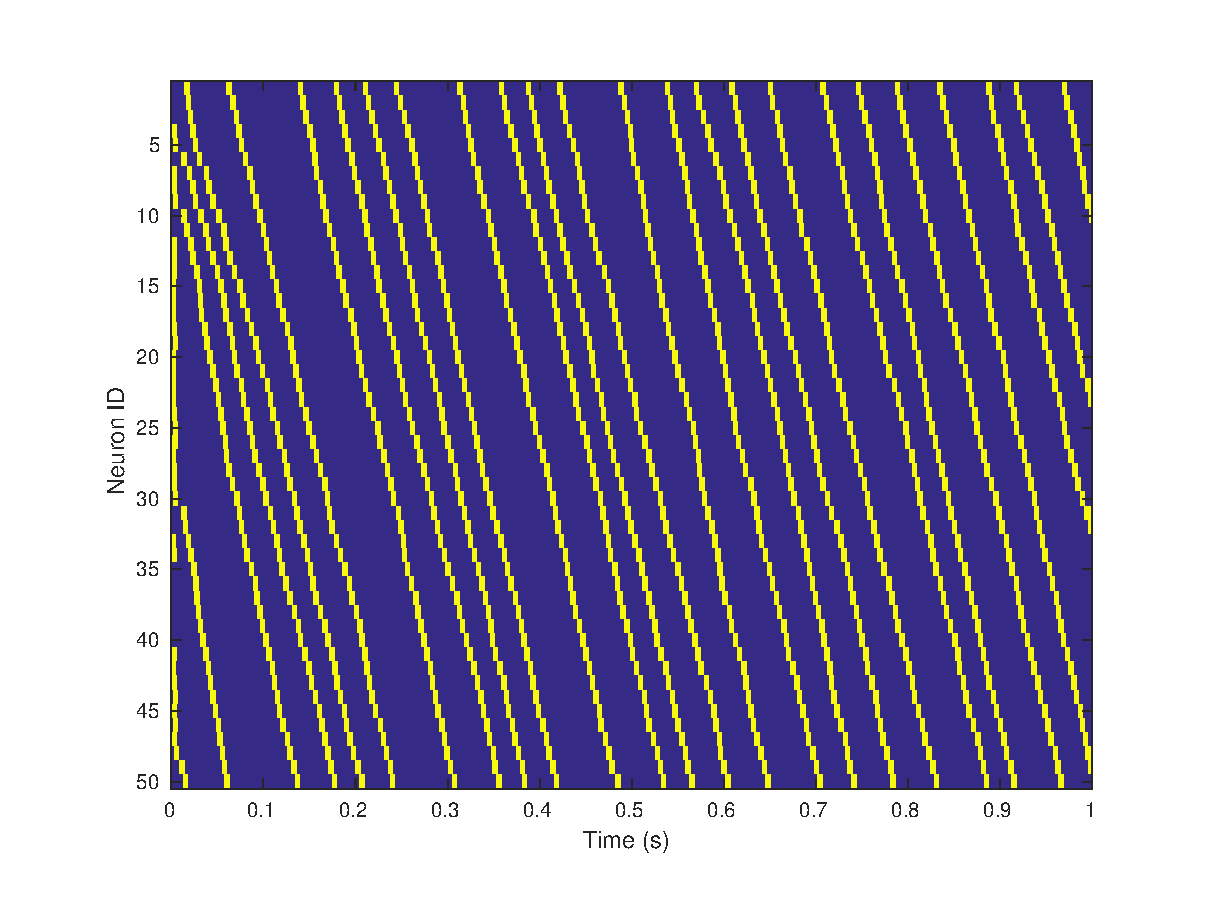
\includegraphics[width = \textwidth]{Burst_nolearning_perm_6000Hz_wmax0.7.eps}
\label{Burst_no_learning: 0.7}
\caption{Bursts without learning, \(w_max = 0.7\).}
\end{subfigure}
\label{Burst_no_learning}
\caption{Compare the four}
\end{figure}
\end{itemize}

\subsection{Convergence and Stability}

\begin{itemize}
\item Demonstrate the stability of our IB model by showing the firing rate plot and how it splits according to \(r_{in}\).

\begin{figure}[H]
\centering
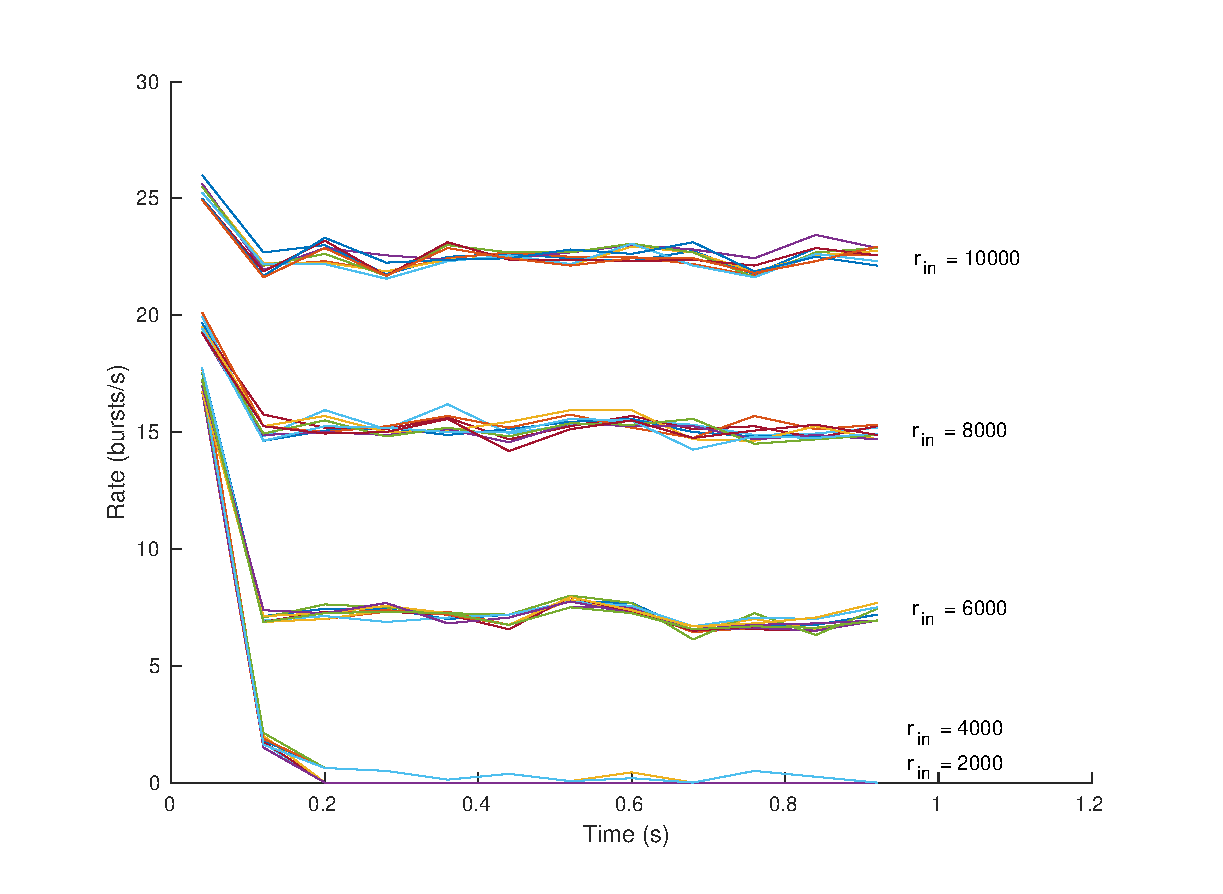
\includegraphics[scale = 0.4]{Firing_Rate_Binsize_80ms.eps}
\label{FR}
\caption{Caption will go here}
\end{figure}

\item Plot Weight and \(WW^T\) for 4000 and 6000 Hz to show some level of convergence.

\begin{figure}[H]
\centering
\begin{subfigure}[b]{0.49\textwidth}
\includegraphics[width = \textwidth]{Weights_4000Hz.eps}
\label{Weights: 4000Hz, basic}
\caption{Weight matrix of 4000Hz annealed}
\end{subfigure}
\,
\begin{subfigure}[b]{0.49\textwidth}
\includegraphics[width = \textwidth]{Weights_6000Hz.eps}
\label{Weights: 6000Hz, basic}
\caption{Weight matrix of 6000Hz annealed}
\end{subfigure}
\\
\begin{subfigure}[b]{0.49\textwidth}
\includegraphics[width = \textwidth]{WW_4000Hz.eps}
\label{Weights: 4000Hz, product}
\caption{\(WW^T\) of 4000Hz annealed}
\end{subfigure}
\,
\begin{subfigure}[b]{0.49\textwidth}
\includegraphics[width = \textwidth]{WW_6000Hz.eps}
\label{Weights: 6000Hz, product}
\caption{\(WW^T\) of 6000Hz annealed}
\end{subfigure}
\label{Weights}
\caption{Compare the four}
\end{figure}

\item Plot error function over time from normal and from permutation matrix

\begin{figure}[H]
\centering
\begin{subfigure}[b]{0.49\textwidth}
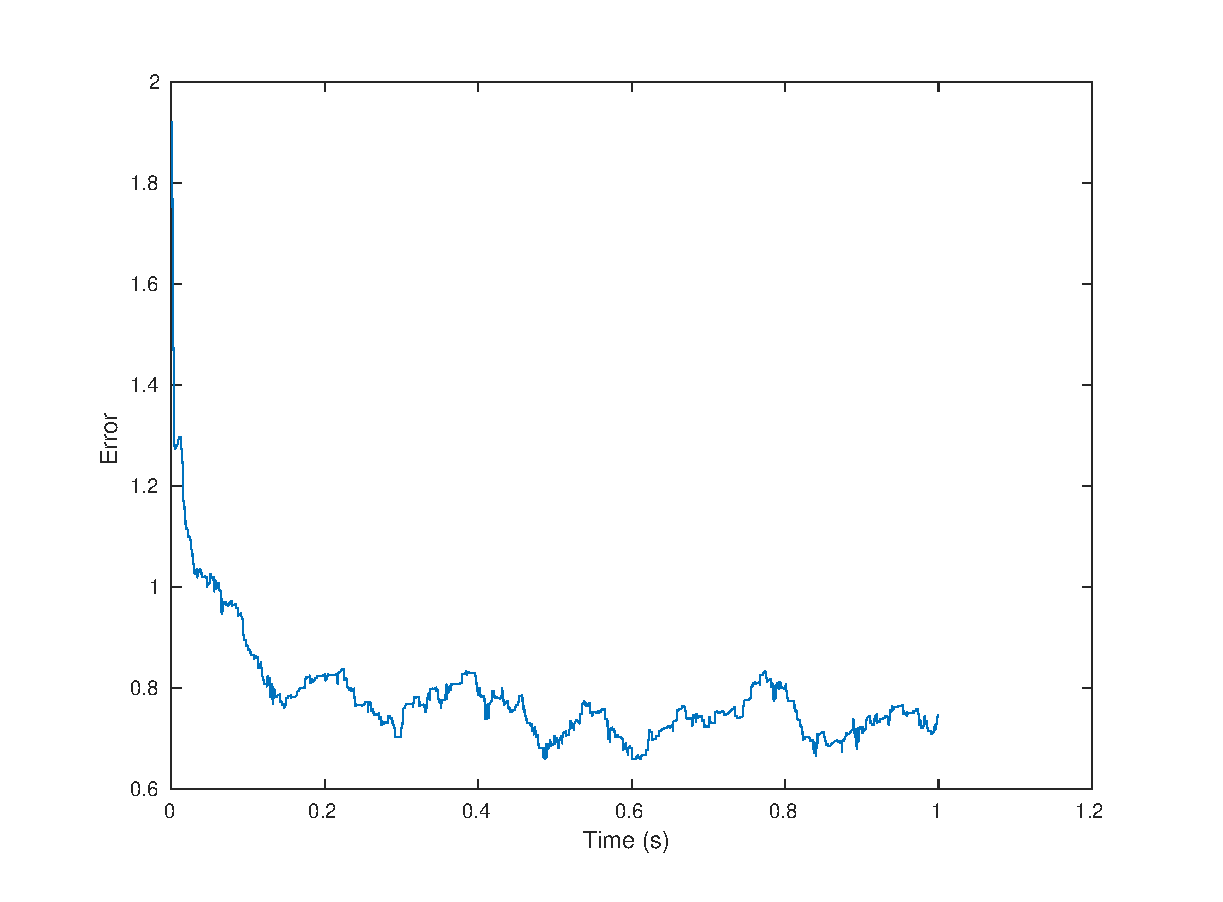
\includegraphics[width = \textwidth]{ErrorOverTime_6000Hz_normal.eps}
\label{Error_over_time: normal}
\caption{Plot of error in weights over time starting from a full connection weight matrix.}
\end{subfigure}
\,
\begin{subfigure}[b]{0.49\textwidth}
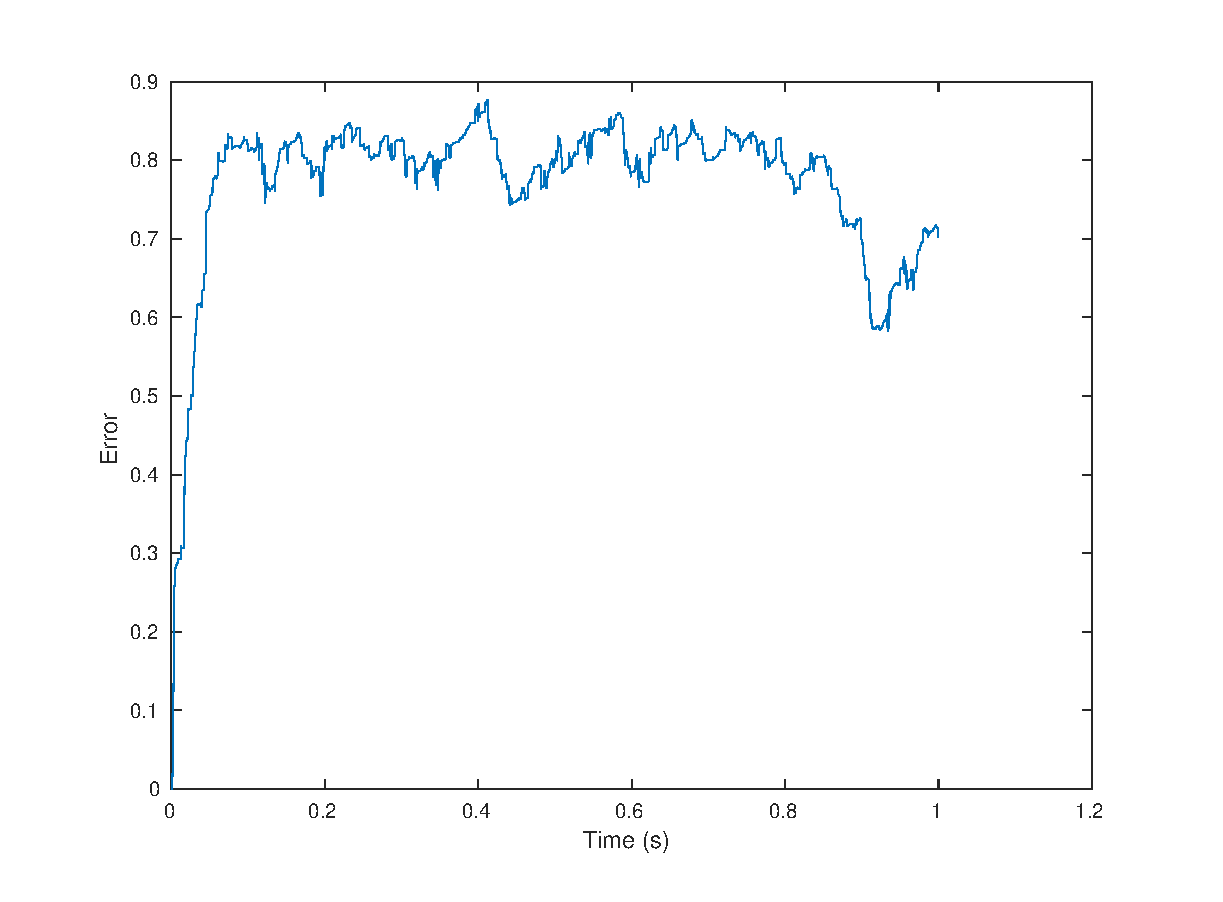
\includegraphics[width = \textwidth]{ErrorOverTime_6000Hz_Perm.eps}
\label{Error_over_time: permutation}
\caption{Plot of error in weights over time starting from a permutation weight matrix.}
\end{subfigure}
\label{Error_over_time}
\caption{Compare the two}
\end{figure}

\item Describe why the error function converges away from (mistake, see discussion).
\end{itemize}

\subsection{Hebbian Learning versus STDP}

\begin{itemize}
\item Introduce the idea of the refutation. 
\item Give a theoretical description why the type of learning should be relatively unimportant.
\item Compare plots (\(WW^T\), Error vs Time, Burst History).

\begin{figure}[H]
\centering
\begin{subfigure}[b]{0.49\textwidth}
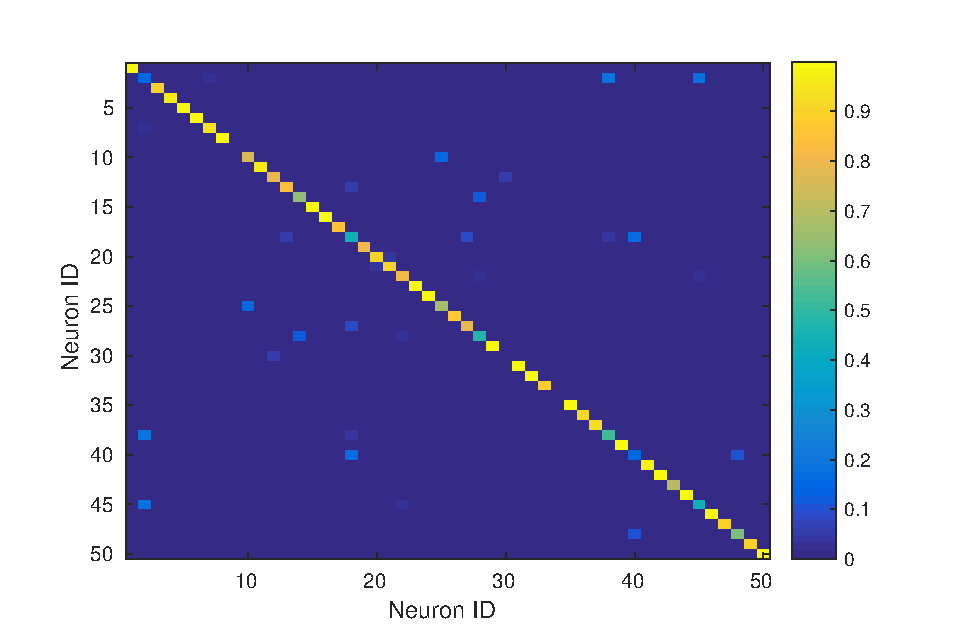
\includegraphics[width = \textwidth]{WW_6000Hz_Hebbian.eps}
\label{Compare: WW_Hebbian}
\caption{Multiplied weight matrix with Hebbian learning}
\end{subfigure}
\,
\begin{subfigure}[b]{0.49\textwidth}
\includegraphics[width = \textwidth]{WW_6000Hz.eps}
\label{Compare: WW_STDP}
\caption{Multiplied weight matrix with STDP learning}
\end{subfigure}
\\
\begin{subfigure}[b]{0.49\textwidth}
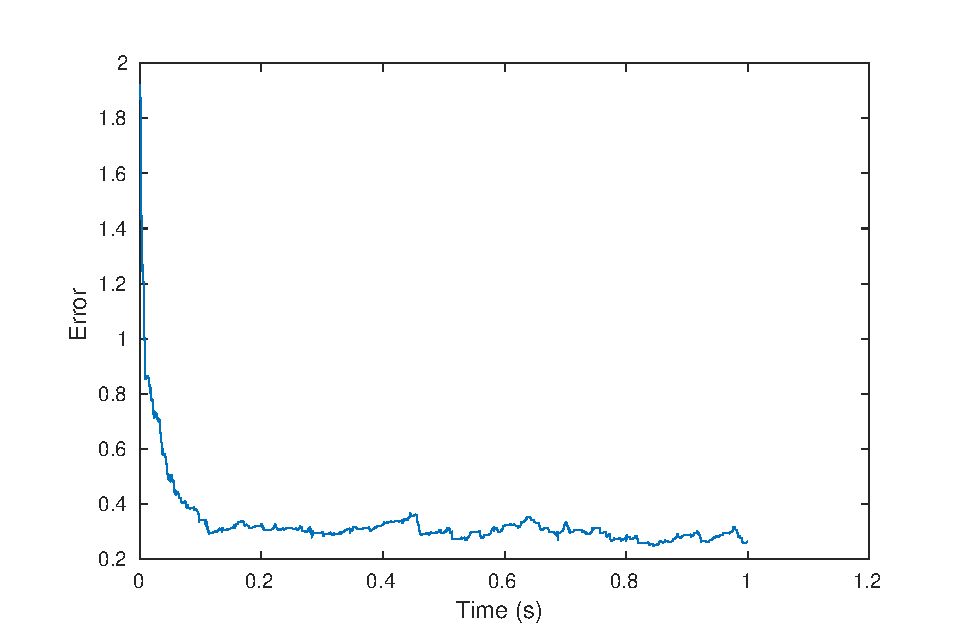
\includegraphics[width = \textwidth]{ErrorOverTime_6000Hz_Hebbian.eps}
\label{Compare: EoT_Hebbian}
\caption{Error over time of Hebbian plot}
\end{subfigure}
\,
\begin{subfigure}[b]{0.49\textwidth}
\includegraphics[width = \textwidth]{WW_6000Hz.eps}
\label{Compare: EoT_STDP}
\caption{Error over time of STDP plot}
\end{subfigure}
\\
\begin{subfigure}[b]{0.49\textwidth}
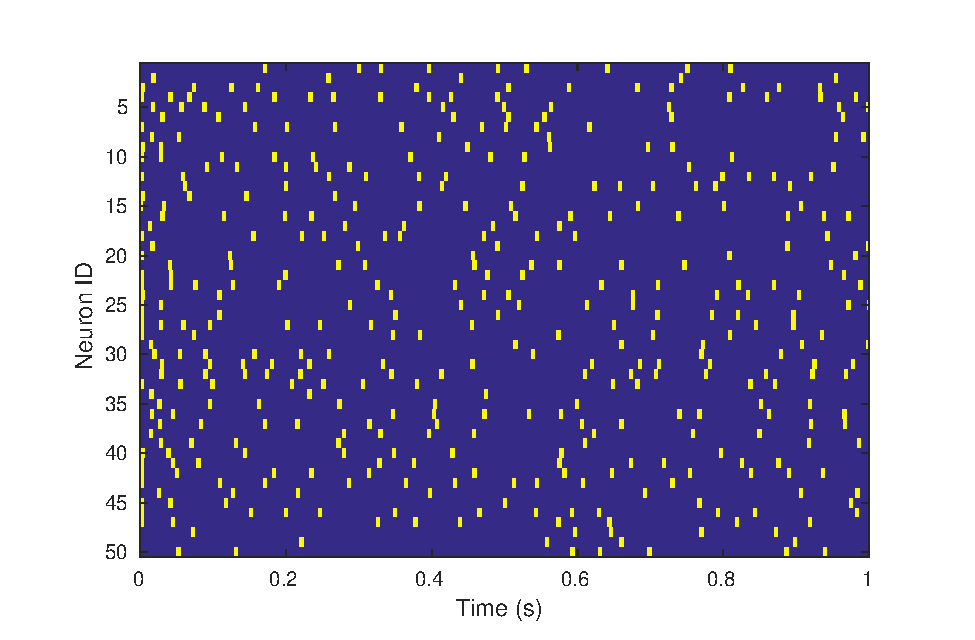
\includegraphics[width = \textwidth]{Burst_plot_6000Hz_Hebbian.eps}
\label{Compare: BH_Hebbian}
\caption{Burst history of Hebbian plot}
\end{subfigure}
\,
\begin{subfigure}[b]{0.49\textwidth}
\includegraphics[width = \textwidth]{Burst_plot_6000Hz.eps}
\label{Compare: BH_STDP}
\caption{Burst history of STDP plot}
\end{subfigure}
\label{Compare}
\caption{Compare STDP to Hebbian}
\end{figure}
\end{itemize}